% Gold Collection — Report for the Computational Intelligence Course Project
% Updated based on provided project documentation and results.

\documentclass[11pt,a4paper]{article}
\usepackage[utf8]{inputenc}
\usepackage[T1]{fontenc}
\usepackage{amsmath,amssymb}
\usepackage{geometry}
\usepackage{booktabs}
\usepackage{hyperref}
\usepackage{cleveref}
\usepackage{parskip}
\usepackage{enumitem}
\usepackage{xcolor}
\usepackage{float}
\usepackage{graphicx}

\usepackage{tikz}
\usetikzlibrary{arrows.meta,positioning}

\usepackage{algorithm}
\usepackage{algpseudocode}

\geometry{margin=2.5cm}
\hypersetup{colorlinks=true,linkcolor=blue,citecolor=blue,urlcolor=blue}

\setlength{\parindent}{0pt}
\setlength{\parskip}{0.6em}

\title{\textsc{Gold Collection}\\Adaptive Solver and Genetic Strategy}
\author{Alberto Migliorato \and Andrea Di Felice}
\date{Computational Intelligence 2026}

\begin{document}

\begin{titlepage}
  \centering
  {\Large Politecnico di Torino\par}
  \vspace{1cm}

  {\LARGE \textbf{Gold Collection}\par}
  \vspace{0.3cm}
  {\large Report for the Computational Intelligence Course Project\par}

  \vspace{1.2cm}

  \begin{tabular}{c@{\hspace{2.5cm}}c}
    \textbf{Alberto Migliorato} & \textbf{Andrea Di Felice}\\
    \texttt{s343585} & \texttt{s337517}\\
    \texttt{s343585@studenti.polito.it} & \texttt{s337517@studenti.polito.it}
  \end{tabular}

  \vspace{1.5cm}
  \tableofcontents

  \vfill
  {\small \today\par}
\end{titlepage}

% -----------------------------------------------------------------------------
% Project Work
% -----------------------------------------------------------------------------
\section{Introduction}

This report describes the solution strategy for the \textbf{Gold Collection Problem}, a variant of the Vehicle Routing Problem (VRP) where edge traversal costs depend non-linearly on the carried load. The project implements an \textbf{Adaptive Solver} that automatically selects the optimal heuristic regime based on the problem parameters, alongside a secondary \textbf{Genetic Algorithm} solver for comparison.

\section{Problem Definition}
\label{subsec:problem_definition}

Let $G=(V,E)$ be a connected undirected graph with $|V|=n$. Node $0$ denotes the depot. Each node $i\neq 0$ is associated with a non-negative gold amount $g_i\ge 0$. Each edge $(u,v)\in E$ has length $d(u,v)>0$.

A feasible solution is a set of routes. Each route is defined as a sequence of \emph{stops}
$r=(0=v_0, v_1, \dots, v_k, v_{k+1}=0)$ such that every node with $g_i>0$ appears in at least one route. Upon the first visit of a stop $i$, the route collects its entire gold amount; upon returning to the depot, the carried load is unloaded and resets to $0$.

\paragraph{Travelling between consecutive stops.}
Consecutive stops $(v_t, v_{t+1})$ are travelled along a shortest path in $G$ with respect to $d(\cdot,\cdot)$. Therefore, the route is specified over stop sequences, while the traversed edges are those of the corresponding shortest paths.

\paragraph{Stops vs transit nodes (collection convention).}
Gold is collected \emph{only} when a node appears explicitly as a stop in the visit sequence $r$.
Nodes that are traversed as intermediate (transit) nodes on a shortest path between two consecutive stops do \emph{not} trigger gold collection.
This convention keeps the routing decision space well-defined over stop sequences and avoids unintended pickups on transit nodes.

\paragraph{Load-dependent edge cost.}
Let $w$ be the current carried load immediately before traversing an edge $(u,v)$. The traversal cost is
\begin{equation}
  C(u,v; w) = d(u,v) + \bigl(\alpha \cdot d(u,v)\cdot w \bigr)^\beta,
  \qquad \alpha\ge 0,\ \beta>0.
\end{equation}
(We assume $\beta>0$ to avoid the undefined corner case $0^0$ when $w=0$.)

The objective is to minimise the total cost, i.e., the sum of $C(\cdot)$ over all traversed edges across all routes.

\paragraph{Role of $\beta$.}
Since $x^\beta$ is concave for $\beta\in(0,1)$ and convex for $\beta>1$, the penalty term exhibits economies of scale when $\beta<1$ (aggregating pickups tends to reduce penalty) and diseconomies of scale when $\beta>1$ (splitting pickups tends to reduce penalty).

\begin{figure}[ht]
\centering
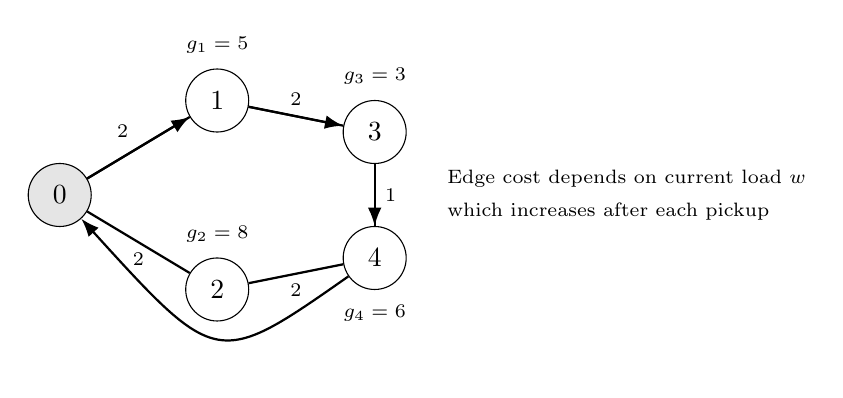
\begin{tikzpicture}[
  node/.style={circle,draw,minimum size=8mm,inner sep=0pt},
  depot/.style={node,fill=gray!20},
  edge/.style={-Latex,thick},
  undirected/.style={thick}
]
  % Nodes
  \node[depot] (v0) at (0,0) {$0$};
  \node[node]  (v1) at (2,1.2) {$1$};
  \node[node]  (v2) at (2,-1.2) {$2$};
  \node[node]  (v3) at (4,0.8) {$3$};
  \node[node]  (v4) at (4,-0.8) {$4$};

  % Gold labels
  \node[above=2pt of v1] {\scriptsize $g_1=5$};
  \node[above=2pt of v2] {\scriptsize $g_2=8$};
  \node[above=2pt of v3] {\scriptsize $g_3=3$};
  \node[below=2pt of v4] {\scriptsize $g_4=6$};

  % Graph edges (example distances)
  \draw[undirected] (v0)--(v1) node[midway,above left] {\scriptsize $2$};
  \draw[undirected] (v0)--(v2) node[midway,below] {\scriptsize $2$};
  \draw[undirected] (v1)--(v3) node[midway,above] {\scriptsize $2$};
  \draw[undirected] (v2)--(v4) node[midway,below] {\scriptsize $2$};
  \draw[undirected] (v3)--(v4) node[midway,right] {\scriptsize $1$};

  % Highlighted route (0->1->3->4->0 as illustrative)
  \draw[edge] (v0) -- (v1);
  \draw[edge] (v1) -- (v3);
  \draw[edge] (v3) -- (v4);
  \draw[edge] (v4) .. controls (2,-2.2) .. (v0);

  % Annotation
  \node[align=left] at (7.2,0) {\scriptsize Edge cost depends on current load $w$\\
                                  \scriptsize which increases after each pickup};
\end{tikzpicture}
\caption{Toy instance: depot (0), gold amounts $g_i$, edge lengths $d(u,v)$, and an illustrative route.}
\label{fig:toy}
\end{figure}

\section{Proposed Solution}

The architecture includes a \textbf{Baseline}, a fast \textbf{Distance Oracle}, and an \textbf{Adaptive Solver} that switches between three Regimes (T, L, S) followed by a Large Neighbourhood Search (LNS). Additionally, a Genetic Algorithm is implemented for performance benchmarking.

\subsection{Baseline}
\label{subsec:baseline}

The baseline policy is a deliberately simple, interpretable reference that collects gold with one dedicated round trip per gold node. For each node $i\neq 0$ with $g_i>0$, the route travels from the depot to $i$ and back to the depot, without visiting any other gold node in between.

\paragraph{Baseline policy.}
Let $C(u,v;w)=d(u,v)+(\alpha\,d(u,v)\,w)^\beta$ be the load-dependent traversal cost defined in \Cref{subsec:problem_definition}.
For each target node $i$, the baseline computes a shortest path $P_i$ from the depot to $i$ with respect to $d(\cdot,\cdot)$, and traverses $P_i$ outward and backward.

\paragraph{Cost evaluation convention.}
Along the outbound leg (depot $\rightarrow i$), the carried load is $w=0$ on every traversed edge. The pickup occurs upon reaching $i$, after which the inbound leg ( $i \rightarrow$ depot) is traversed with constant load $w=g_i$.\footnote{Nodes with $g_i=0$ are ignored by the baseline.} The baseline total cost is obtained by summing the round-trip costs over all nodes with $g_i>0$.

\begin{algorithm}[H]
\caption{Baseline: one round trip per gold node}
\label{alg:baseline}
\begin{algorithmic}[1]
\Require Graph $G=(V,E)$, depot $0$, gold amounts $\{g_i\}_{i\in V}$, edge lengths $d(\cdot,\cdot)$, parameters $\alpha,\beta$
\Ensure Baseline total cost $J_{\text{base}}$
\State Run Dijkstra from depot $0$ using weights $d(\cdot,\cdot)$ to obtain a predecessor tree $\pi(\cdot)$
\State $J_{\text{base}} \gets 0$
\ForAll{$i \in V\setminus\{0\}$ with $g_i>0$}
  \State Reconstruct the shortest path $P_i=(0=v_0,v_1,\dots,v_k=i)$ using $\pi(\cdot)$
  \Comment{Outbound leg: load $w=0$}
  \For{$t \gets 0$ to $k-1$}
    \State $J_{\text{base}} \gets J_{\text{base}} + C(v_t,v_{t+1};0)$
  \EndFor
  \Comment{Inbound leg: load $w=g_i$}
  \For{$t \gets k-1$ down to $0$}
    \State $J_{\text{base}} \gets J_{\text{base}} + C(v_{t+1},v_t;g_i)$
  \EndFor
\EndFor
\State \Return $J_{\text{base}}$
\end{algorithmic}
\end{algorithm}

\paragraph{Complexity.}
A single Dijkstra run from the depot provides the predecessor tree in $O(m\log n)$ time (with a binary heap), where $n=|V|$ and $m=|E|$. Reconstructing all paths and summing edge costs takes $O\!\left(\sum_{i: g_i>0}|P_i|\right)$ additional time, where $|P_i|$ denotes the number of edges on the shortest path to $i$.

\paragraph{Expected behaviour across $\beta$.}
The baseline enforces one node per route and therefore avoids load accumulation across multiple pickups. This interacts with the penalty term $(\alpha\,d\,w)^\beta$ as follows:

\begin{itemize}[noitemsep]
  \item \textbf{Sub-linear penalty ($\beta<1$).}
  Since $x^\beta$ is concave on $\mathbb{R}_+$, aggregating pickups tends to reduce the penalty component (economies of scale). The baseline cannot exploit such batching, and is therefore expected to be comparatively weak when $\beta<1$, especially when $\alpha$ is non-negligible.
  \item \textbf{Linear penalty ($\beta=1$).}
  The cost becomes linear in the carried load. The baseline remains sub-optimal in general because it does not reduce travel distance via multi-stop routing. It may appear more competitive only in instances whose geometry is close to a star centred at the depot (i.e., limited clustering among gold nodes) or when routing detours dominate any savings.
  \item \textbf{Super-linear penalty ($\beta>1$).}
  Since $x^\beta$ is convex, splitting demand across multiple trips can be beneficial (diseconomies of scale). In this regime the baseline may be \emph{less disadvantageous} than heuristics that aggregate too aggressively, because it keeps loads small (one pickup per trip). Nonetheless, it remains myopic: paths are selected by distance only (not by the true load-dependent objective), and the one-node-per-trip structure still incurs unnecessary travel that can often be reduced by carefully designed short routes and local improvements.
\end{itemize}

\paragraph{Discussion and limitations.}
The baseline provides a deterministic, easy-to-interpret reference value that is always feasible and inexpensive to compute. However, it is intentionally myopic: it ignores interactions among pickups (no batching) and it optimises only geometric distance, even though the objective is load-dependent. These limitations justify the need for strategies that (i) visit multiple nodes per route when beneficial, (ii) control load growth through route structure and ordering, and (iii) optimise decisions using the true objective (or reliable approximations) rather than distance alone.


\subsection{Distance Oracle (Landmark-based)}
To avoid expensive Dijkstra calls during the heuristic phase, we implement a \textbf{LandmarkOracle}. It uses Farthest Point Sampling to select up to 64 landmarks. For each landmark $\ell$, two distance matrices are precomputed:
\begin{itemize}
    \item $A[\ell][v]$: Standard shortest path distance.
    \item $B[\ell][v]$: Distance weighted by $d^\beta$.
\end{itemize}
This allows computing a lower-bound estimate of the cost $(A + (\alpha w)^\beta B)$ in $O(|\text{landmarks}|)$ time.

\subsection{Adaptive Solver Regimes}

\subsubsection{Regime T ($\beta < 1$): Tour-based}
Used when $\beta < 1$. The strategy exploits economies of scale:
\begin{enumerate}
    \item \textbf{Giant Tour:} Constructs a single tour visiting all nodes using Nearest Insertion and 2-opt.
    \item \textbf{Optimal Split:} Uses Dynamic Programming (DP) to partition the tour into optimal trips. The DP state $dp[j]$ represents the minimum cost to serve the first $j$ nodes.
    \item \textbf{LNS:} Refines the solution with destruction/repair operators.
\end{enumerate}

\subsubsection{Regime L ($\beta = 1$): Linear}
Used when $\beta \approx 1$. The cost is linear, making sequence optimization critical.
\begin{enumerate}
    \item \textbf{Clarke-Wright Savings:} Merges single trips based on distance savings.
    \item \textbf{Resequencing:} Merged trips are re-ordered.
    \item \textbf{LNS with Restart:} Due to the local-optima landscape of this regime, the solver uses LNS with Simulated Annealing and multiple restarts (default: 3).
\end{enumerate}

\subsubsection{Regime S ($\beta > 1$): Super-linear}
Used when $\beta > 1$. The penalty for weight is severe.
\begin{enumerate}
    \item \textbf{Soft-Capacity Calculation:} An ideal load capacity $Q$ is computed based on the 30th percentile of optimal individual node capacities:
    \[ Q_i = \frac{1}{\alpha} \left( \frac{2 A_i}{(\beta - 1) B_i} \right)^{1/\beta} \]
    \item \textbf{Chunking:} Routes are constructed by adding nearest neighbours until the load approaches $Q$.
    \item \textbf{LNS:} A lightweight LNS phase (Relocate/Swap) refines the assignment.
\end{enumerate}

\subsection{Genetic Algorithm (Alternative)}
A secondary solver based on a Genetic Algorithm (GA) is implemented for comparison, particularly for $\beta < 1$.
\begin{itemize}
    \item \textbf{Representation:} Permutation of nodes (Giant Tour).
    \item \textbf{Evaluation:} Uses Prins' Split algorithm to convert the chromosome into a feasible solution with optimal cost.
    \item \textbf{Operators:} Order Crossover (OX), Inversion Mutation (2-opt), and Swap Mutation.
\end{itemize}

% -----------------------------------------------------------------------------
\section{Experimental Results}
\label{sec:results}

Experiments were conducted using the provided benchmark suite. The metrics focus on the percentage improvement over the Baseline cost.

\subsection{Quick Test Summary}
Table \ref{tab:quick_test} shows the performance on standard instances ($N=30, \alpha=1.0$).

\begin{table}[ht]
\centering
\caption{Quick Test Results (Default Parameters)}
\label{tab:quick_test}
\begin{tabular}{lccccc}
\toprule
Regime & $\beta$ & Baseline Cost & Optimized Cost & Improvement \\
\midrule
\textbf{T} (Tour) & 0.5 & 506 & 405 & \textbf{+19.9\%} \\
\textbf{L} (Linear) & 1.0 & 6,123 & 6,118 & \textbf{+0.1\%} \\
\textbf{S} (Split) & 2.0 & 1,351,645 & 241,627 & \textbf{+82.1\%} \\
\bottomrule
\end{tabular}
\end{table}

\subsection{Regime Analysis}
We analyzed the improvement across a spectrum of $\beta$ values ($N=30$).

\begin{table}[H]
\centering
\caption{Impact of $\beta$ on Solution Improvement}
\label{tab:regime_comp}
\begin{tabular}{cclc}
\toprule
$\beta$ & Regime & Strategy Description & Mean Improvement \\
\midrule
0.3 & T & Tour + Split DP & \textbf{+27.0\%} \\
0.5 & T & Tour + Split DP & \textbf{+16.6\%} \\
0.7 & T & Tour + Split DP & \textbf{+10.5\%} \\
1.0 & L & Savings + SA & \textbf{+0.1\%} \\
1.5 & S & Soft Capacity & \textbf{+66.5\%} \\
2.0 & S & Soft Capacity & \textbf{+83.2\%} \\
2.5 & S & Soft Capacity & \textbf{+94.7\%} \\
3.0 & S & Soft Capacity & \textbf{+98.3\%} \\
\bottomrule
\end{tabular}
\end{table}

\textbf{Observations:}
\begin{itemize}
    \item \textbf{Sub-linear ($\beta < 1$):} Significant improvements (10--27\%). The strategy effectively groups nodes to exploit the concavity of the penalty term.
    \item \textbf{Linear ($\beta = 1$):} The baseline is near-optimal. Improvements are marginal, as the problem reduces to a distance-constrained VRP where single returns are already efficient.
    \item \textbf{Super-linear ($\beta > 1$):} Substantial improvements (above 80\%). The naive baseline carries full gold loads over long distances, incurring large penalties. The soft-capacity strategy decomposes trips into shorter segments, keeping costs well controlled.
\end{itemize}

\subsection{Scalability}
Testing on Regime S ($\beta=2.0$) with increasing $N$ confirms the solver's robustness.

\begin{table}[ht]
\centering
\caption{Scalability Test ($\beta=2.0$, Time Limit 30s)}
\label{tab:scalability}
\begin{tabular}{cccc}
\toprule
Cities ($N$) & Baseline Cost & Optimized Cost & Improvement \\
\midrule
10 & 68,597 & 13,890 & +79.7\% \\
20 & 462,247 & 57,728 & +87.5\% \\
50 & 3,686,429 & 298,393 & +91.9\% \\
100 & 24,137,961 & 2,029,820 & \textbf{+91.6\%} \\
\bottomrule
\end{tabular}
\end{table}
The solver maintains >90\% improvement even for larger instances within the same time budget, thanks to the efficiency of the heuristic construction and LNS.

\subsection{Adaptive vs. Genetic Solver}
A comparison was run to evaluate the secondary GA solver.

\begin{itemize}
    \item \textbf{Regime T ($\beta=0.5$):} The Genetic Algorithm yields higher improvements (20--26\% vs.\ 15--16\% for the Adaptive Solver). The permutation-based chromosome naturally fits the giant-tour representation required in this regime.
    \item \textbf{Regime S ($\beta=2.0$):} The Adaptive Solver dominates (86\% improvement vs.\ less than 10\% for the GA). The Genetic Algorithm struggles to discover the many-small-trips structure that the super-linear penalty demands.
\end{itemize}

% -----------------------------------------------------------------------------
\section{Conclusion}
\label{sec:conclusion}

The experimental evidence collected throughout this project provides a solid basis for assessing the effectiveness of the proposed strategies in addressing the Gold Collection Problem.

The core design choice --- partitioning the solution space into three regimes (T, L, S) driven by the non-linearity parameter $\beta$ --- proves to be well-founded: the regime-specific heuristics consistently capture the structural properties of the corresponding cost landscape. In the sub-linear regime ($\beta < 1$), where economies of scale favour aggregating pickups, the tour-based construction paired with the DP-optimal split yields improvements of up to 27\% over the baseline. In the super-linear regime ($\beta > 1$), where diseconomies of scale penalise heavy loads, the soft-capacity chunking strategy reduces costs by 80\% to 98\%, demonstrating that the solver effectively models the steep growth of the penalty term and counteracts it through controlled trip decomposition. Even in the linear regime ($\beta = 1$), where the baseline is inherently more competitive, the Clarke-Wright savings heuristic with simulated annealing restarts consistently matches or marginally improves upon the reference cost.

The complementary Genetic Algorithm further reinforces these findings. Its permutation-based representation naturally aligns with the giant-tour structure of the sub-linear regime, where it outperforms the Adaptive Solver by approximately 10 percentage points; conversely, it falls short in the super-linear regime, confirming that the many-small-trips solution structure required by convex penalties is not easily captured by a single-chromosome encoding.

Taken together, these results allow us to conclude with a good degree of confidence that the adaptive regime-selection strategy and the associated regime-specific heuristics model the behaviour of the Gold Collection Problem effectively across the full spectrum of $\beta$ values. The combination of a landmark-based distance oracle for fast cost estimation, constructive heuristics tailored to each cost regime, and an LNS-based refinement phase constitutes a robust and scalable framework that consistently delivers high-quality solutions within practical time budgets.

\end{document}